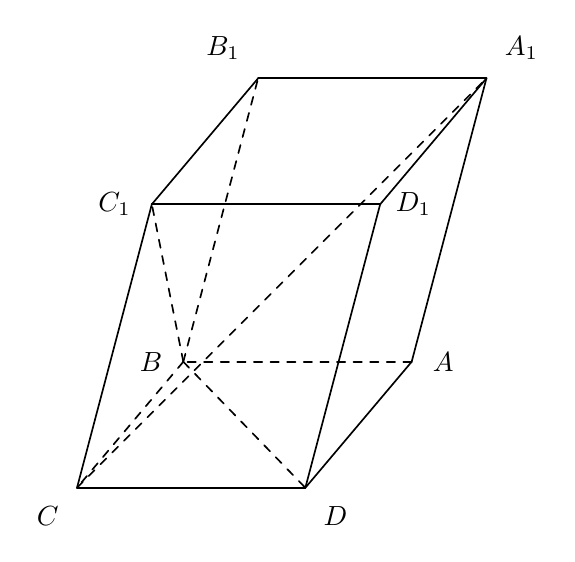
\begin{tikzpicture}[line width=0.6pt, line join=round, line cap=round, font=\normalsize]
  % oblique parallelepiped: C origin
  \coordinate (C) at (0,0);
  \coordinate (D) at (2.9,0);
  \coordinate (Bm) at (1.35,1.6);
  \coordinate (Am) at (4.25,1.6);
  \coordinate (C1) at (0.95,3.6);
  \coordinate (D1) at (3.85,3.6);
  \coordinate (B1) at (2.3,5.2);
  \coordinate (A1) at (5.2,5.2);
  % bottom face
  \draw (C) -- (D);
  \draw (D) -- (Am);
  \draw[dashed] (Am) -- (Bm);
  \draw[dashed] (Bm) -- (C);
  % top face
  \draw (C1) -- (D1);
  \draw (D1) -- (A1);
  \draw (A1) -- (B1);
  \draw (B1) -- (C1);
  % laterals
  \draw (C) -- (C1);
  \draw (D) -- (D1);
  \draw (Am) -- (A1);
  \draw[dashed] (Bm) -- (B1);
  % hidden diagonals from B
  \draw[dashed] (Bm) -- (D);
  \draw[dashed] (Bm) -- (C1);
  % space diagonal C-A1
  \draw[dashed] (C) -- (A1);
  % diagonal C1-B already via Bm-C1; add Bm-A1 dashed (part of space diagonal region)
  
  % labels with clearance
  \node[below left=3pt] at (C) {$C$};
  \node[below right=3pt] at (D) {$D$};
  \node[left=4pt] at (Bm) {$B$};
  \node[right=4pt] at (Am) {$A$};
  \node[left=4pt] at (C1) {$C_{1}$};
  \node[right=2pt] at (D1) {$D_{1}$};
  \node[above left=3pt] at (B1) {$B_{1}$};
  \node[above right=3pt] at (A1) {$A_{1}$};
\end{tikzpicture}
